% Created 2024-01-24 Τετ 18:01
% Intended LaTeX compiler: pdflatex
\documentclass[11pt]{article}
\usepackage[utf8]{inputenc}
\usepackage[T1]{fontenc}
\usepackage{graphicx}
\usepackage{longtable}
\usepackage{wrapfig}
\usepackage{rotating}
\usepackage[normalem]{ulem}
\usepackage{amsmath}
\usepackage{amssymb}
\usepackage{capt-of}
\usepackage{hyperref}
\usepackage{booktabs}
\usepackage{import}
\usepackage[LGR, T1]{fontenc}
\usepackage[greek, english, american]{babel}
\usepackage{alphabeta}
\usepackage{esint}
\usepackage{mathtools}
\usepackage{esdiff}
\usepackage{makeidx}
\usepackage{glossaries}
\usepackage{newfloat}
\usepackage{minted}
\usepackage[a4paper, margin=3cm]{geometry}
\usepackage{chemfig}
\usepackage{svg}
\author{Vidianos Giannitsis}
\date{\today}
\title{Hypothesis testing and sensitivity analysis of Hydrolysis HPLC data}
\hypersetup{
 pdfauthor={Vidianos Giannitsis},
 pdftitle={Hypothesis testing and sensitivity analysis of Hydrolysis HPLC data},
 pdfkeywords={},
 pdfsubject={},
 pdfcreator={Emacs 29.1 (Org mode 9.6.6)}, 
 pdflang={English}}
\makeatletter
\newcommand{\citeprocitem}[2]{\hyper@linkstart{cite}{citeproc_bib_item_#1}#2\hyper@linkend}
\makeatother

\usepackage[notquote]{hanging}
\begin{document}

\maketitle
\tableofcontents

\begin{abstract}
Έχουμε πάρει πολλά δεδομένα από την HPLC για διάφορες συγκεντρώσεις σε κάθε πείραμα. Ένα καλό ερώτημα το οποίο δεν έχουμε εξετάσει είναι κατά πόσο είναι στατιστικά σημαντική η προσθήκη του μιξ γενικά ή και ξεχωριστά από το ένα επίπεδο στο άλλο. Σκοπός του αρχείου αυτού είναι να εξετάσει κάτι τέτοιο με χρήση της ANOVA. Έπειτα, αν δούμε ότι η επίδραση είναι σημαντική μπορούμε να προχωρήσουμε και σε μία ανάλυση ευαισθησίας για να δούμε και ποσότικα πόσο επηρεάζει, εκτός από ποιοτικά.
\end{abstract}

\section{Dependencies}
\label{sec:org18cd2f6}
Αρχικά, όπως και στα άλλα notebooks, πρέπει να κάνουμε load κάποια dependencies τα οποία θα χρειαστούμε για αυτό το code base.

\begin{minted}[breaklines=true,breakanywhere=true]{julia}

using DrWatson
@quickactivate "Masters_Thesis"
include(srcdir("filenames.jl"))
using CSV, DataFrames, Statistics, Distributions

\end{minted}

\section{Φόρτωση των δεδομένων}
\label{sec:org504ddc4}
Έπειτα, πρέπει να διαβάσουμε τα CSVs με τα δεδομένα για να μπορέσουμε να κάνουμε την ανάλυση μας.

\begin{minted}[breaklines=true,breakanywhere=true]{julia}

# Read all the data
exp_35 = "10_11"
exp_40 = "28_11"
exp_45 = "23_10"
mix_amount = ["0", "1", "2", "4", "8"]

# Experiment @35 C
df35_0 = CSV.read(get_conc_csv(exp_35, mix_amount[1]), DataFrame)
df35_1 = CSV.read(get_conc_csv(exp_35, mix_amount[2]), DataFrame)
df35_2 = CSV.read(get_conc_csv(exp_35, mix_amount[3]), DataFrame)
df35_4 = CSV.read(get_conc_csv(exp_35, mix_amount[4]), DataFrame)
df35_8 = CSV.read(get_conc_csv(exp_35, mix_amount[5]), DataFrame)

# Experiment @40 C
df40_0 = CSV.read(get_conc_csv(exp_40, mix_amount[1]), DataFrame)
df40_1 = CSV.read(get_conc_csv(exp_40, mix_amount[2]), DataFrame)
df40_2 = CSV.read(get_conc_csv(exp_40, mix_amount[3]), DataFrame)
df40_4 = CSV.read(get_conc_csv(exp_40, mix_amount[4]), DataFrame)
df40_8 = CSV.read(get_conc_csv(exp_40, mix_amount[5]), DataFrame)

# Experiment @45 C
df45_1 = CSV.read(get_conc_csv(exp_45, mix_amount[2]), DataFrame)
df45_2 = CSV.read(get_conc_csv(exp_45, mix_amount[3]), DataFrame)
\end{minted}

\section{Επεξεργασία πρωτογενών δεδομένων}
\label{sec:org8c3bad6}
Βέβαια, δεν θέλουμε αυτούς τους πίνακες. Αρχικά θέλουμε να συγκρίνουμε τις 5 ποσότητες σε κάθε θερμοκρασία, οπότε θέλουμε τα vector των τελικών συγκεντρώσεων κάθε ένωσης.

\begin{minted}[breaklines=true,breakanywhere=true]{julia}

# Take the maximum instead of defaulting for the last element as we
# know ethanol is consumed so the last isn't the maximum which is the
# one we are interested in.
prod35_0 = map(maximum, eachcol(df35_0[:, 5:8]))
prod35_1 = map(maximum, eachcol(df35_1[:, 5:8]))
prod35_2 = map(maximum, eachcol(df35_2[:, 5:8]))
prod35_4 = map(maximum, eachcol(df35_4[:, 5:8]))
prod35_8 = map(maximum, eachcol(df35_8[:, 5:8]))

prod40_0 = map(maximum, eachcol(df40_0[:, 5:8]))
prod40_1 = map(maximum, eachcol(df40_1[:, 5:8]))
prod40_2 = map(maximum, eachcol(df40_2[:, 5:8]))
prod40_4 = map(maximum, eachcol(df40_4[:, 5:8]))
prod40_8 = map(maximum, eachcol(df40_8[:, 5:8]))

prod_35 = hcat(prod35_0, prod35_1, prod35_2, prod35_4, prod35_8)
prod_40 = hcat(prod40_0, prod40_1, prod40_2, prod40_4, prod40_8)

# Collect the 4 vectors which have the output variable in every condition
lact_mean_35 = prod_35[1,:]
acet_mean_35 = prod_35[2,:]
prop_mean_35 = prod_35[3,:]
eth_mean_35 = prod_35[4,:]

lact_mean_40 = prod_40[1,:]
acet_mean_40 = prod_40[2,:]
prop_mean_40 = prod_40[3,:]
eth_mean_40 = prod_40[4,:]

# For the sensitivity analysis, we want to compare both variables
# simultaneously, so we group the two prod vectors.
prod = hcat(prod35_0, prod35_1, prod35_2, prod35_4, prod35_8, prod40_0, prod40_1, prod40_2, prod40_4, prod40_8)

lact = prod[1,:]
acet = prod[2,:]
prop = prod[3,:]
eth = prod[4,:]
\end{minted}

\section{Visualization των αποτελεσμάτων αυτών}
\label{sec:org8980b58}
Για να είναι πιο ευπαρουσίαστα τα αποτελέσματα της ανάλυσης, αξίζει να κάνουμε κάποια διαγράμματα που δείχνουν την τελική συγκέντρωση της κάθε ένωσης ανάλογα με το mix amount.

\begin{minted}[breaklines=true,breakanywhere=true]{julia}

using Plots

xtick = ["0", "1", "2", "4", "8"]
plot_label = ["Lactate" "Acetate" "Propionate" "Ethanol"]

prod_scatter_35 = scatter(1:5, [lact_mean_35 acet_mean_35 prop_mean_35 eth_mean_35],
                          xticks = (1:5, ["0", "1", "2", "4", "8"]),
                          xlabel = "Mix Amount (ml)", ylabel = "Concentration (g/l)",
                          markersize = 6, label = plot_label,
                          title = "Product Concentration by mix amount - 35 C")
savefig(plotsdir("10_11", "final_prod_scatter_10_11.png"))

prod_scatter_40 = scatter(1:5, [lact_mean_40 acet_mean_40 prop_mean_40 eth_mean_40],
                          xticks = (1:5, ["0", "1", "2", "4", "8"]),
                          xlabel = "Mix Amount (ml)", ylabel = "Concentration (g/l)",
                          markersize = 6, label = plot_label,
                          title = "Product Concentration by mix amount - 40 C")
savefig(plotsdir("28_11", "final_prod_scatter_28_11.png"))

\end{minted}

\begin{center}
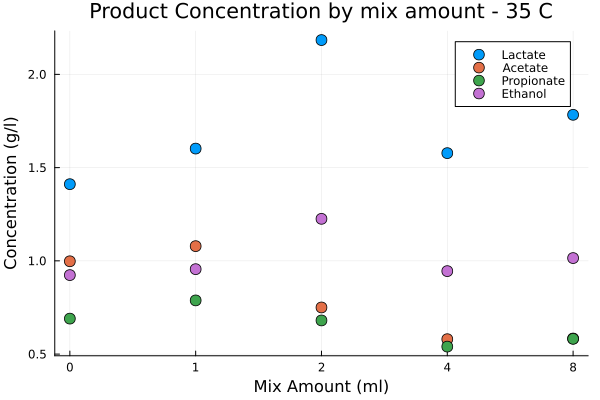
\includegraphics[width=.9\linewidth]{../plots/10_11/final_prod_scatter_10_11.png}
\end{center}

\begin{center}
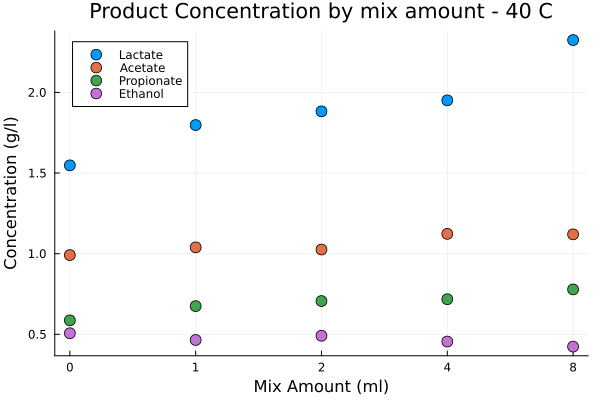
\includegraphics[width=.9\linewidth]{../plots/28_11/final_prod_scatter_28_11.png}
\end{center}

\section{Δημιουργία ψευδο-κατανομής των δεδομένων}
\label{sec:org5e9d411}
Για να κάνουμε ANOVA χρειάζεται κάθε μέτρηση να έχει ένα sample size μεγαλύτερο του 1 (και εφόσον κάνουμε στατιστική ανάλυση, τυπικά θέλουμε πάνω από 5 για στατιστικά σημαντικά αποτελέσματα). Δεν μπορούμε να κάνουμε το πείραμα τόσες φορές, οπότε χρειαζόμαστε έναν μηχανισμό για να φτιάξουμε δεδομένα.

Ένα claim το οποίο δεν είναι κακό είναι ότι αν κάναμε πολλές φορές το πείραμα, τα αποτελέσματα θα ακολουθούσαν κανονική κατανομή. Οπότε, με έναν μέσο όρο και μία τυπική απόκλιση, μπορούμε να φτιάξουμε δεδομένα τα οποία θα είναι περίπου σωστά και να τρέξουμε με αυτά την ANOVA. Οι μέσοι όροι θα είναι προφανώς οι τιμές που θα έχουμε παρατηρήσει. Για τις τυπικές αποκλίσεις θέλουμε κάτι άλλο. Από τα συγκεκριμένα πειράματα δεν μπορούμε να βγάλουμ κάπως ακριβής τυπική απόκλιση. Όμως, έχουμε το προπαρασκευαστικό πείραμα που έγινε στους 45 C στο οποίο είχαμε 2 επαναλήψεις και συχνή δειγματοληψία. Μπορούμε (με ένα σφάλμα) να πάρουμε την τυπική απόκλιση των 6 τιμών οι οποίες είναι κοντινές μεταξύ τους και να υποθέσουμε ότι μία παρόμοια τιμή θα έχει και η τυπική απόκλιση αυτών που μας ενδιαφέρουν.

\subsection{Pre-processing}
\label{sec:org06f33c9}
Για να πάρουμε τα δεδομένα ακολουθούμε μία παρόμοια λογική με παραπάνω και μόλις βρούμε τα διανύσματα που θέλουμε υπολογίζουμε τo standard deviation τους.

\begin{minted}[breaklines=true,breakanywhere=true]{julia}

prod45_1 = select(df45_1, 1, 5:8)
prod45_2 = select(df45_2, 1, 5:8)

# Day 0
d0_prod = vcat(prod45_1[2:7, 2:5], prod45_2[1:3, 2:5])
# The first point in the first data has some very noticeable outliers
# that will massively increase the deviation if included.
std_d0 = std.(eachcol(d0_prod))

# Day 1
d1_prod = vcat(Vector(prod45_1[8, 2:5])', Vector(prod45_1[10, 2:5])', Vector(prod45_2[6, 2:5])')
# The times 24 and 26 hours in the second experiment are before
# Glucose is fully consumed and have much lower products than those in
# the other experiment, hence there cannot be a standard deviation
# including them. For 26 hours in the first experiment, Lactate has a
# weird increase that is lost within 2 hours, which is considered a
# possible outlier in this case.
std_d1 = [std(d1_prod[:,i]) for i in 1:4]

# Day 2

# Day 3
\end{minted}

\subsection{Δημιουργία των κατανομών}
\label{sec:orgc3fa595}
Έχοντας την τυπική απόκλιση και τον μέσο όρο μπορούμε να φτιάξουμε τις κατανομές. Χάριν ευκολίας, θα φτιαχτούν vectorized κατανομές.

\begin{minted}[breaklines=true,breakanywhere=true]{julia}

lact_dist_35 = [Normal(lact_mean_35[i], lact_std_35) for i in 1:length(lact_mean_35)]
acet_dist_35 = [Normal(acet_mean_35[i], acet_std_35) for i in 1:length(acet_mean_35)]
prop_dist_35 = [Normal(prop_mean_35[i], prop_std_35) for i in 1:length(prop_mean_35)]
eth_dist_35 = [Normal(eth_mean_35[i], eth_std_35) for i in 1:length(eth_mean_35)]

lact_dist_40 = [Normal(lact_mean_40[i], lact_std_40) for i in 1:length(lact_mean_40)]
acet_dist_40 = [Normal(acet_mean_40[i], acet_std_40) for i in 1:length(acet_mean_40)]
prop_dist_40 = [Normal(prop_mean_40[i], prop_std_40) for i in 1:length(prop_mean_40)]
eth_dist_40 = [Normal(eth_mean_40[i], eth_std_40) for i in 1:length(eth_mean_40)]

\end{minted}

\subsection{Sampling}
\label{sec:org4de1b17}
Έχοντας τις κατανομές, μπορούμε να κάνουμε sample έναν αριθμό από δείγματα για να τρέξουμε την ANOVA. Εφόσον έχουμε την δυνατότητα να πάρουμε όσα samples θέλουμε, μπορούμε να βάλουμε και μεγάλα νούμερα, αλλά για παράδειγμα 20 δείγματα είναι μάλλον ένα καλό νούμερο.

\begin{minted}[breaklines=true,breakanywhere=true]{julia}

samples = 20
lact_samples_35 = [rand(lact_dist_35[i], samples) for i in 1:length(lact_mean_35)]
acet_samples_35 = [rand(acet_dist_35[i], samples) for i in 1:length(acet_mean_35)]
prop_samples_35 = [rand(prop_dist_35[i], samples) for i in 1:length(prop_mean_35)]
eth_samples_35 = [rand(eth_dist_35[i], samples) for i in 1:length(eth_mean_35)]

lact_samples_40 = [rand(lact_dist_40[i], samples) for i in 1:length(lact_mean_40)]
acet_samples_40 = [rand(acet_dist_40[i], samples) for i in 1:length(acet_mean_40)]
prop_samples_40 = [rand(prop_dist_40[i], samples) for i in 1:length(prop_mean_40)]
eth_samples_40 = [rand(eth_dist_40[i], samples) for i in 1:length(eth_mean_40)]

\end{minted}

\section{ANOVA}
\label{sec:org9b52ddd}
Έχοντας κάνει sample έχουμε τώρα κάποια διανύσματα όπου τα καθένα έχει 20 παρατηρήσεις και μπορεί να γίνει μία ANOVA για να δείξει σε ποιά από τα 8 συστήματα (4 προιόντα, 2 θερμοκρασίες) έπαιξε όντως ρόλο η προσθήκη του μιξ και σε ποιά δεν φαίνεται να έπαιξε. Αρχικά, γράφουμε ένα function που κάνει implement την ANOVA.

\begin{minted}[breaklines=true,breakanywhere=true]{julia}

<<dependencies>>
include(scriptsdir("hypothesis_sensitivity_preprocessing.jl"))

function manualANOVA(allData)
    nArray = length.(allData)
    d = length(nArray)

    xBarTotal = mean(vcat(allData...))
    xBarArray = mean.(allData)

    ssBetween = sum( [nArray[i]*(xBarArray[i] - xBarTotal)^2 for i in 1:d] )
    ssWithin = sum([sum([(ob - xBarArray[i])^2 for ob in allData[i]])
                                for i in 1:d])
    dfBetween = d-1
    dfError = sum(nArray)-d

    msBetween = ssBetween/dfBetween
    msError = ssWithin/dfError
    fStat = msBetween/msError
    pval = ccdf(FDist(dfBetween,dfError),fStat)
    return fStat, pval
end

\end{minted}

και έπειτα το εφαρμόζουμε στα 8 διανύσματα που παράξαμε πριν. Το output θα είναι η τιμή του f-statistic καθώς και το p-value. Τυπικά σε μία ANOVA, αν το f-statistic είναι κοντά στο 1 δεν μπορούμε να απορρίψουμε την υπόθεση H\textsubscript{0} η οποία λέει πως δεν έπαιξε ρόλο η προσθήκη του mix αλλά έγινε τυχαία. Το p-value μας λέει με τι βεβαιότητα απορρίπτουμε ή όχι την υπόθεση.

\begin{minted}[breaklines=true,breakanywhere=true]{julia}

lact_anova_35 = manualANOVA(lact_samples_35)
acet_anova_35 = manualANOVA(acet_samples_35)
prop_anova_35 = manualANOVA(prop_samples_35)
eth_anova_35 = manualANOVA(eth_samples_35)

lact_anova_40 = manualANOVA(lact_samples_40)
acet_anova_40 = manualANOVA(acet_samples_40)
prop_anova_40 = manualANOVA(prop_samples_40)
eth_anova_40 = manualANOVA(eth_samples_40)

anova_35 = reshape([lact_anova_35..., acet_anova_35..., prop_anova_35..., eth_anova_35...], 2, 4)
anova_40 = reshape([lact_anova_40..., acet_anova_40..., prop_anova_40..., eth_anova_40...], 2, 4)

\end{minted}

Από τα αποτελέσματα αυτά, είναι εμφανές πως η ποσότητα του mix που προστίθεται είναι σίγουρα σημαντική επειδή όλα τα p-values είναι πάρα πολύ χαμηλά.

Μπορούμε επίσης να τα αποθηκεύσουμε σε έναν ωραίο πίνακα:

\begin{minted}[breaklines=true,breakanywhere=true]{julia}

names = ["Lactate_35", "Acetate_35", "Propionate_35", "Ethanol_35", "Lactate_40", "Acetate_40", "Propionate_40", "Ethanol_40"]
anova_data = hcat(anova_35, anova_40)

anova_table = Tables.table(hcat(names, anova_data'), header = [:Test, :FStatistic, :pValue])
CSV.write(datadir("exp_pro", "anova_35_40.csv"), anova_table)
DataFrame(anova_table)

\end{minted}

\section{Άλλα hypothesis tests}
\label{sec:org93719f2}
\subsection{ANOVA σε 2 mL και πάνω}
\label{sec:org4fae339}
Από τα διαγράμματα που είχαμε κάνει, είχε παρατηρηθεί πως ενδέχεται να μην έχει νόημα να βάλουμε πάνω από 2 ml του mix. Στους 35, η συμπεριφορά που παρατηρήθηκε ήταν καθαρά αρνητική ενώ στους 40 σε πολλά φάνηκε να είναι περίπου αμελητέα αν όχι αρνητική. Οπότε, έχει νόημα να κάνουμε anova και εδώ για να δούμε τι βγάζει.

\begin{minted}[breaklines=true,breakanywhere=true]{julia}

lact_anova_35_2plus = manualANOVA(lact_samples_35[3:5])
acet_anova_35_2plus = manualANOVA(acet_samples_35[3:5])
prop_anova_35_2plus = manualANOVA(prop_samples_35[3:5])
eth_anova_35_2plus = manualANOVA(eth_samples_35[3:5])

lact_anova_40_2plus = manualANOVA(lact_samples_40[3:5])
acet_anova_40_2plus = manualANOVA(acet_samples_40[3:5])
prop_anova_40_2plus = manualANOVA(prop_samples_40[3:5])
eth_anova_40_2plus = manualANOVA(eth_samples_40[3:5])

anova_35_2plus = reshape([lact_anova_35_2plus..., acet_anova_35_2plus..., prop_anova_35_2plus..., eth_anova_35_2plus...], 2, 4)
anova_40_2plus = reshape([lact_anova_40_2plus..., acet_anova_40_2plus..., prop_anova_40_2plus..., eth_anova_40_2plus...], 2, 4)

anova_data_2plus = hcat(anova_35_2plus, anova_40_2plus)

anova_table_2plus = Tables.table(hcat(names, anova_data_2plus'), header = [:Test, :FStatistic, :pValue])
CSV.write(datadir("exp_pro", "anova_35_40_2plus.csv"), anova_table_2plus)
DataFrame(anova_table_2plus)

\end{minted}

\begin{verbatim}
2×4 Matrix{Float64}:
 390.101        5.21984     4.37956    145.021
   5.51787e-34  0.00828594  0.0170094    4.38079e-23
\end{verbatim}


Προκύπτει πως στους 35 όλες οι μεταβολές είναι στατιστικά σημαντικές και είναι όλες μειώσεις. Οπότε σίγουρα δεν θέλουμε πάνω από 2 ml. Στους 40, η αιθανόλη μειώνεται με στατιστικά σημαντικό τρόπο ενώ το γαλακτικό αυξάνεται. Το οξικό και το προπιονικό και αυτά αυξάνονται με στατιστικά σημαντικό τρόπο, αλλά έχουν πολύ μεγαλύτερα p-values. Συγκεκριμένα το οξικό μπορούμε να απορρίψουμε την H\textsubscript{0} με confidence interval 99\% αλλά οριακά και στο προπιονικό μπορούμε με interval 95\%. Οπότε στους 40 υπάρχει επαρκής evidence για να πάμε σε πάνω από 2 ml.

\subsection{T-test για 4-8 ml στους 40}
\label{sec:orgcb8ade1}
Εφόσον στους 40 υπάρχει evidence για να πάμε πάνω από 2 ml, αξίζει να δούμε και αν υπάρχει evidence για να πάμε στα 8 ml ή αν δεν είναι στατιστικά σημαντικό σε σχέση με το 4.

\begin{minted}[breaklines=true,breakanywhere=true]{julia}

lact_ttest_40 = EqualVarianceTTest(lact_samples_40[4], lact_samples_40[5])
acet_ttest_40 = EqualVarianceTTest(acet_samples_40[4], acet_samples_40[5])
prop_ttest_40 = EqualVarianceTTest(prop_samples_40[4], prop_samples_40[5])
eth_ttest_40 = EqualVarianceTTest(eth_samples_40[4], eth_samples_40[5])

ttest_40_res = [pvalue(lact_ttest_40), pvalue(acet_ttest_40), pvalue(prop_ttest_40), pvalue(eth_ttest_40)]
\end{minted}

Τα αποτελέσματα του test αυτού δείχνουν πως η αλλαγή του οξικού και του προπιονικού δεν είναι στατιστικά σημαντική (το οξικό με μεγάλη βεβαιότητα, το προπιονικό οριακά δεν μπορεί να απορριφθεί στο 95\%) ενώ η αιθανόλη μειώνεται με στατιστικά σημαντικό τρόπο. Οπότε, αν σκεφτούμε το αυξημένο κόστος της προσθήκης μεγαλύτερης ποσότητας, αφού επηρεάζεται μόνο το γαλακτικό, δεν είναι στατιστικά σημαντική η προσθήκη 8 ml σε αντίθεση με τα 4.

\subsection{ANOVA σε 2 ml και κάτω}
\label{sec:orgc7bd2e4}
Εφόσον στους 35 δεν έχει νόημα να πάμε πάνω από 2, αξίζει να εξεταστεί αν έχει νόημα και το 2 ή μήπως ούτε αυτό χρειάζεται και θα λειτουργούσε το ίδιο και χωρίς ένζυμα. Χάριν ευκολίας, εξετάζουμε το ίδιο ερώτημα και για τους 40, παρόλο που έκει έχουμε δείξει ότι το 4 ml είναι σημαντικά καλύτερο από το 2 και αναμένουμε ότι κάτι παρόμοιο θα ισχύει και εδώ.

\begin{minted}[breaklines=true,breakanywhere=true]{julia}

lact_anova_35_2minus = manualANOVA(lact_samples_35[1:3])
acet_anova_35_2minus = manualANOVA(acet_samples_35[1:3])
prop_anova_35_2minus = manualANOVA(prop_samples_35[1:3])
eth_anova_35_2minus = manualANOVA(eth_samples_35[1:3])

lact_anova_40_2minus = manualANOVA(lact_samples_40[1:3])
acet_anova_40_2minus = manualANOVA(acet_samples_40[1:3])
prop_anova_40_2minus = manualANOVA(prop_samples_40[1:3])
eth_anova_40_2minus = manualANOVA(eth_samples_40[1:3])

anova_35_2minus = reshape([lact_anova_35_2minus..., acet_anova_35_2minus..., prop_anova_35_2minus..., eth_anova_35_2minus...], 2, 4)
anova_40_2minus = reshape([lact_anova_40_2minus..., acet_anova_40_2minus..., prop_anova_40_2minus..., eth_anova_40_2minus...], 2, 4)

anova_data_2minus = hcat(anova_35_2minus, anova_40_2minus)

anova_table_2minus = Tables.table(hcat(names, anova_data_2minus'), header = [:Test, :FStatistic, :pValue])
CSV.write(datadir("exp_pro", "anova_35_40_2minus.csv"), anova_table_2minus)
DataFrame(anova_table_2minus)

\end{minted}

Για τους 35, προκύπτει με πολύ μεγάλη βεβαιότητα ότι οι μεταβολές που υπάρχουν μεταξύ αυτών των 3 ποσοτήτων είναι στατιστικά σημαντικές. Βέβαια, το οξικό και το προπιονικό μειώνονται με στατιστικά σημαντικό τρόπο, δεν αυξάνονται.

Για τους 40, προκύπτει πως δεν μπορούμε σε καμία περίπτωση να πούμε ότι το οξικό αυξάνεται με στατιστικά σημαντικό τρόποστην περιοχή αυτή. Όπως είδαμε παραπάνω, επίσης ρόλο δεν παίζει η μεταβολή από 4 σε 8 ml. Οπότε στην πράξη, η μόνη αλλαγή που έπαιξε ρόλο στην συγκέντρωση του οξικού ήταν αυτή από τα 2 στα 4 ml που ούτε αυτή έπαιξε μεγάλο ρόλο.

\subsection{Επίδραση της θερμοκρασίας}
\label{sec:orge31d411}
Εκτός από τα παραπάνω που έδειξαν ότι οι διαφορετικές παίζουν ρόλο και ανάλογα με το τι θέλουμε επιλέγουμε ποια θα πάρουμε, έχει νόημα να εξετάσουμε και αν είναι στατιστικά σημαντική η επίδραση της θερμοκρασίας. Για αυτό, πρέπει να κάνουμε t-test μεταξύ ίδιων ποσοτήτων στις 2 θερμοκρασίες. Ο κώδικας για αυτό είναι παρακάτω.

\begin{minted}[breaklines=true,breakanywhere=true]{julia}

# Run the hypothesis tests
lact_temp_ttest = [UnequalVarianceTTest(lact_samples_35[i], lact_samples_40[i]) for i in 1:length(lact_samples_35)]
acet_temp_ttest = [UnequalVarianceTTest(acet_samples_35[i], acet_samples_40[i]) for i in 1:length(acet_samples_35)]
prop_temp_ttest = [UnequalVarianceTTest(prop_samples_35[i], prop_samples_40[i]) for i in 1:length(prop_samples_35)]
eth_temp_ttest = [UnequalVarianceTTest(eth_samples_35[i], eth_samples_40[i]) for i in 1:length(eth_samples_35)]

# Get the pvalues of each test
lact_temp_pvalues = pvalue.(lact_temp_ttest)
acet_temp_pvalues = pvalue.(acet_temp_ttest)
prop_temp_pvalues = pvalue.(prop_temp_ttest)
eth_temp_pvalues = pvalue.(eth_temp_ttest)

# Format them in a nice table and write it to CSV
temp_ttest_table = Tables.table(hcat(mix_amount, lact_temp_pvalues, acet_temp_pvalues, prop_temp_pvalues, eth_temp_pvalues), header = [:Mix_Amount, :Lactate, :Acetate, :Propionate, :Ethanol])
CSV.write(datadir("exp_pro", "temp_ttest.csv"), temp_ttest_table)
DataFrame(temp_ttest_table)
\end{minted}

Από τα αποτελέσματα, είναι εμφανές πως η θερμοκρασία παίζει ρόλο παντού. Αξίζει να σημειωθεί πως σε 2 τιμές του οξικού και μία του προπιονικού, ο ρόλος της θερμοκρασίας δεν είναι σίγουρος, αλλά με 95\% βεβαιότητα μπορούμε να απορρίψουμε την υπόθεση ότι δεν παίζει ρόλο παντού.

\section{Τελικά συμπεράσματα από τα hypothesis tests}
\label{sec:org6a0261d}
Στο αρχείο αυτό έγιναν διάφορα hypothesis tests με σκοπό να δούμε αν οι παραμέτροι που ελέγχουμε έχουν στατιστικά σημαντική επίδραση στην τελική συγκέντρωση των προιόντων. Σε γενικές γραμμές, οι περισσότερες παραμέτροι έχουν σημαντική επίδραση, καθώς σε ελάχιστες περιπτώσεις δεν μπορούσε να απορριφθεί η υπόθεση H\textsubscript{0}. Σε κάποιες περιπτώσεις όμως, αυτό το συμπέρασμα δεν μπορεί να βγεί με τόση βεβαιότητα.

Τα τεστ που έγιναν είναι τα εξής: ANOVA μεταξύ των 5 διαφορετικών ποσοτήτων mix στις 2 δύο θερμοκρασίες και στα 4 προιόντα. ANOVA μεταξύ των ποσοτήτων 2, 4 και 8 ml και στις 2 θερμοκρασίες για να δούμε αν πραγματικά επιφέρει κάτι η προσθήκη πάνω από 2 ml. t-test μεταξύ 4 και 8 ml στους 40 (όπου είχε νόημα να αυξήσουμε πάνω από 2 ml με βάση το προηγούμενο). ANOVA μεταξύ 0, 1 και 2 ml στους 35 για να δούμε αν έχουν νόημα τα 2 ml επειδή τα παραπάνω σίγουρα δεν έχουν. t-test συγκρίνοντας τις 2 θερμοκρασίες για κάθε mix\textsubscript{amount} και ένωση.

Καθώς οι περισσότερες υποθέσεις απορρίφθηκαν με μεγάλη βεβαιότητα (μεγαλύτερη από 99.99\%), παρακάτω θα σημειωθούν όσες απορρίφθηκαν με λιγότερη ή δεν μπόρεσαν να απορριφθούν.

\subsection{Απόρριψη με 99\% βεβαιότητα}
\label{sec:org0f18935}
Το οξικό στους 40 για ποσότητες 2-8 ml.
Το t-test για την θερμοκρασία στα 0 ml οξικού.

\subsection{Απόρριψη με 95\% βεβαιότητα}
\label{sec:orgdf394ff}
Το προπιονικό στους 40 για ποσότητες 2-8 ml.
Το t-test για την θερμοκρασία στο 1 ml οξικό και στα 2 ml προπιονικό.

\subsection{Δεν μπόρεσαν να απορριφθούν}
\label{sec:org4557597}
Το οξικό στους 40 για ποσότητες 0-2 ml.
Το t-test για το οξικό και το προπιονικό στους 40 μεταξύ 4 και 8 ml.

Οπότε, το τελικό συμπέρασμα είναι πως στους 35, υπάρχει ευαισθησία σε όλο το εύρος των ποσοτήτων που βάλαμε, αλλά στα 2 ml φαίνεται να λειτουργεί καλύτερα από ότι σε παραπάνω. Στους 40, τα 4 ml δείχνουν να έχουν την καλύτερη λειτουργία καθώς αποτελούν βελτίωση από τα 2 ml και δεν είναι στατιστικά σημαντική η βελτίωση αν πάμε στα 8 ml για 2 από τις 4 ενώσεις, ενώ η μία (αιθανόλη) μειώνεται κιόλας. Βέβαια, για τις δύο ενώσεις αυτές, η αύξηση από τα 2 στα 4 ml είναι οριακά στατιστικά σημαντική (με 95\% βεβαιότητα στο προπιονικό και 99\% στο οξικό) και αν λάβουμε υπόψην το κόστος, πιθανόν και αυτό να μην αξίζει. Από άποψη θερμοκρασίας, το οξικό στα 0 και 1 ml είναι αρκετά παρόμοιο και στις δύο θερμοκρασίες, παρόλο που με 99 και 95\% βεβαιότητα αντίστοιχα μπορούμε να πούμε πως είναι διαφορετικά. 

\section{Ανάλυση Ευαισθησίας}
\label{sec:orga5b2a11}
Έχοντας δει κάποια ποιοτικά συμπεράσματα από την ANOVA παραπάνω και γνωρίζοντας πλέον ότι σχεδόν όλες οι μεταβολές είναι στατιστικά σημαντικές, μπορούμε να προχωρήσουμε σε ποσοτικά αποτελέσματα και να δούμε πόσο επηρεάζει η κάθε παράμετρος πραγματικά. Αυτό μπορεί να γίνει με ανάλυση ευαισθησίας. Για να τρέξουμε την ανάλυση ευαισθησίας ως προς τις δύο παραμέτρους λειτουργίας, χρειαζόμαστε για κάθε ένωση μία συνάρτηση η οποία παίρνει ένα διάνυσμα των δύο μεταβλητών και δίνει μία προβλεπόμενη συγκέντρωση. Από τα πειράματα, έχουμε 10 διαφορετικά σημεία για 5 ποσότητες μιξ και 2 θερμοκρασίες. Μεταξύ των σημείων δεν έχουμε κάποιο δεδομένο, οπότε η μόνη προσέγγιση που μπορούμε να κάνουμε είναι πως συνδέουμε γραμμικά τα σημεία. Αυτό ενέχει ένα σφάλμα σίγουρα, αλλά είναι η καλύτερη δυνατή προσέγγιση που μπορεί να γίνει. Ως κομμάτι του preprocessing, θα γίνει και αυτό tangled στο ίδιο αρχείο με τα παραπάνω, καθώς χρησιμοποιεί και τα ίδια δεδομένα.

\begin{minted}[breaklines=true,breakanywhere=true]{julia}

using Interpolations, GlobalSensitivity

nodes = ([0.0, 1.0, 2.0, 4.0, 8.0], [35, 40])
lact_itp = interpolate(nodes, reshape(lact, 5, 2), Gridded(Linear()))
acet_itp = interpolate(nodes, reshape(acet, 5, 2), Gridded(Linear()))
prop_itp = interpolate(nodes, reshape(prop, 5, 2), Gridded(Linear()))
eth_itp = interpolate(nodes, reshape(eth, 5, 2), Gridded(Linear()))

function lact_interp(x)
    lact_itp(x[1], x[2])
end

function acet_interp(x)
    acet_itp(x[1], x[2])
end

function prop_interp(x)
    prop_itp(x[1], x[2])
end

function eth_interp(x)
    eth_itp(x[1], x[2])
end

\end{minted}

Έπειτα, μπορούμε να τρέξουμε την ανάλυση ευαισθησίας σε όλη την πειραματική περιοχή ή σε κάποια subdomain της. Αρχικά, το αρχείο του sensitivity analysis πρέπει να έχει τα dependencies και να κάνει include το preprocessing.

\begin{minted}[breaklines=true,breakanywhere=true]{julia}

<<dependencies>>
include(scriptsdir("hypothesis_sensitivity_preprocessing.jl"))

\end{minted}

To GlobalSensitivity.jl προσφέρει δύο είδη ανάλυσης ευαισθησίας. Το πρώτο, βασίζεται στη μέθοδο Morris, η οποία είναι μία στοχαστική μέθοδος που υπολογίζει την παράγωγο της συνάρτησης ως προς τις παραμέτρους της (το οποίο τον ορισμό της ευαισθησίας) αριθμητικά, αλλά με μεγάλα βήματα. Έτσι, δεν υπολογίζει ακριβής παραγώγους, αλλά μέσες τιμές αυτής σε μεγάλο εύρος. Με πολλές επαναλήψεις, αυτή η μέθοδος πετυχαίνει μία καλή προσέγγιση της παραγώγου. Λόγω της στοχαστικής φύσης της όμως, παρόλο που κάθε τρέξιμο της συνάρτησης έχει από μόνο του πολλές επαναλήψεις, καλό είναι να την τρέξουμε πολλές φορές και να πάρουμε ένα μέσο όρο των μέσων όρων για να έχει επαναληψιμότητα αυτό που κάνουμε. Χάριν ευκολίας για την επεξεργασία των δεδομένων αποθηκεύουμε ένα vector με τα 4 vectors ευαισθησιών (ένα για κάθε ένωση). Αυτό φαίνεται παρακάτω.

\begin{minted}[breaklines=true,breakanywhere=true]{julia}

function morris_sens_analysis(bounds)
    sens_mean_vector = []
    for i in 1:200
        lact_sens = gsa(lact_interp, Morris(), bounds)

        acet_sens = gsa(acet_interp, Morris(), bounds)

        prop_sens = gsa(prop_interp, Morris(), bounds)

        eth_sens = gsa(eth_interp, Morris(), bounds)

        push!(sens_mean_vector, [lact_sens.means, acet_sens.means, prop_sens.means, eth_sens.means])
    end

    return mean(sens_mean_vector)
end

\end{minted}

Η άλλη μέθοδος που χρησιμοποιείται συχνά είναι η μέθοδος Sobol. Η μέθοδος αυτή βασίζεται στην ίδια λογική με την ANOVA, ότι μπορούμε σπάσουμε την συνολική μεταβλητότητα της συνάρτησης σε διάφορους παράγοντες. Στην περίπτωση της μεθόδου Sobol, σπάμε τη μεταβλητότητα σε μεταβλητότητα λόγω της κάθε μεταβλητής ξεχωριστά και έπειτα σε αλληλεπιδράσεις τους. Στην περίπτωση των 2 μεταβλητών υπάρχουν μόνο 3 όροι, οι δύο μεταβλητές ξεχωριστά και η αλληλεπίδραση τους. Το αποτέλεσμα που δίνει η μέθοδος αυτή είναι τα Sobol indices που δείχνουν τον λόγο της μεταβλητότητας ως προς μία μεταβλητή προς την συνολική μεταβλητότητα. Στην περίπτωση μας, χρειαζόμαστε μόνο τα first order indices καθώς η αλληλεπίδραση αποτελεί το 1-το άθροισμα των άλλων δύο, αφού το άθροισμα των επιμέρους μεταβλητοτήτων πρέπει να είναι η συνολική μεταβλητότητα. Η εφαρμογή της είναι η εξής

\begin{minted}[breaklines=true,breakanywhere=true]{julia}

function sobol_sens_analysis(bounds)
    lact_sens = gsa(lact_interp, Sobol(), bounds, samples = 500)
    acet_sens = gsa(acet_interp, Sobol(), bounds, samples = 500)
    prop_sens = gsa(prop_interp, Sobol(), bounds, samples = 500)
    eth_sens = gsa(eth_interp, Sobol(), bounds, samples = 500)

    S1_res = hcat(lact_sens.S1, acet_sens.S1, prop_sens.S1, eth_sens.S1)
end

\end{minted}

\subsection{Εφαρμογή της ανάλυσης ευαισθησίας}
\label{sec:org56b0b68}
Έχοντας γράψει τα παραπάνω, μπορούμε να ορίσουμε διάφορα domains και να τρέξουμε σε αυτά την ανάλυση. Εκτός από το συνολικό domain, έχει ενδιαφέρον να κοιτάξουμε τις περιοχές των χαμηλών και υψηλών ποσοτήτων του mix (0 εώς 2 και 2 εώς 8) για να ενισχύσουμε περαιτέρω την υπόθεση μας ότι από 0 εώς 2 έχουμε ισχυρές θετικές επιδράσεις ενώ από 2 εώς 8 ελαφρώς θετικές ή και αρνητικές. Επίσης, έχει ενδιαφέρον να προσπαθήσουμε να δούμε την επίδραση του mix amount στα δύο επίπεδα θερμοκρασίας πιο συγκεκριμένα, καθώς μπορεί να δώσει διαφορετικά συμπεράσματα από τα παραπάνω. Αυτό το τελευταίο δεν έχει νόημα να συμπεριληφθεί στην ανάλυση Sobol, καθώς εκεί θα βγεί ότι στο domain αυτό το 99.999\% της μεταβλητότητας εξαρτάται από το mix amount ή κάτι παρόμοιο.

\begin{minted}[breaklines=true,breakanywhere=true]{julia}

sens_bounds = [[0,8],[35,40]]
sens_bound_35 = [[0,8],[35,35.1]]
sens_bound_40 = [[0,8],[39.9,40]]
sens_bound_low = [[0,2],[35,40]]
sens_bound_high = [[2, 8],[35,40]]

total_sens = morris_sens_analysis(sens_bounds)
sens_35 = morris_sens_analysis(sens_bound_35)
sens_40 = morris_sens_analysis(sens_bound_40)
sens_low = morris_sens_analysis(sens_bound_low)
sens_high = morris_sens_analysis(sens_bound_high)

total_sens_sobol = sobol_sens_analysis(sens_bounds)
sens_low_sobol = sobol_sens_analysis(sens_bound_low)
sens_high_sobol = sobol_sens_analysis(sens_bound_high)

\end{minted}

Έπειτα, αλλάζουμε λίγο τα δεδομένα, για να είναι πιο εύκολο να γίνουν visualized, για να τα ερμηνεύσουμε. Αυτό θα γίνει με χρήση του CairoMakie, ενός πολύ καλού visualization library.

\begin{minted}[breaklines=true,breakanywhere=true]{julia}

# For the Morris sensitivity analysis, we need one Matrix instead of
# Vectors of vectors for each data set. Furthermore, the data from the
# sensitivity analyses in the two temperatures, don't need to be
# plotted separately, as its going to be one row each, compared to the
# others being two rows (one for mix amount sensitivity and one for
# temperature).
total_sens2 = vcat(total_sens[1], total_sens[2], total_sens[3], total_sens[4])
sens_35_2 = vcat(sens_35[1], sens_35[2], sens_35[3], sens_35[4])[:,1]
sens_40_2 = vcat(sens_40[1], sens_40[2], sens_40[3], sens_40[4])[:,1]
sens_temp = hcat(sens_35_2, sens_40_2)
sens_low2 = vcat(sens_low[1], sens_low[2], sens_low[3], sens_low[4])
sens_high2 = vcat(sens_high[1], sens_high[2], sens_high[3], sens_high[4])

# For the Sobol data, we just want to add a column containing the
# interaction, which for this system can be 1 - the sum of the other
# terms.
total_sens_sobol_data = vcat(total_sens_sobol, [1 - sum(total_sens_sobol[:, i]) for i in 1:4]')
sens_low_sobol_data = vcat(sens_low_sobol, [1 - sum(sens_low_sobol[:, i]) for i in 1:4]')
sens_high_sobol_data = vcat(sens_high_sobol, [1 - sum(sens_high_sobol[:, i]) for i in 1:4]')

\end{minted}

Πριν το visualization όμως, μπορούμε να αποθηκεύσουμε τα δεδομένα σε CSVs για εύκολο access. Τα δεδομένα θα αποθηκευτούν στα processed experimental data στο datadir.

\begin{minted}[breaklines=true,breakanywhere=true]{julia}

names = ["Mix Amount", "Temperature", "Interaction"]

# Save the data of the Morris analysis
total_sens_morris_table = Tables.table(hcat(names[1:2], total_sens2'), header = [:Variable, :Lactate, :Acetate, :Propionate, :Ethanol])
CSV.write(datadir("exp_pro", "total_sens_morris.csv"), total_sens_morris_table)
total_sens_morris_df = DataFrame(total_sens_morris_table)

sens_low_morris_table = Tables.table(hcat(names[1:2], sens_low2'), header = [:Variable, :Lactate, :Acetate, :Propionate, :Ethanol])
CSV.write(datadir("exp_pro", "sens_low_morris.csv"), sens_low_morris_table)
sens_low_morris_df = DataFrame(sens_low_morris_table)

sens_high_morris_table = Tables.table(hcat(names[1:2], sens_high2'), header = [:Variable, :Lactate, :Acetate, :Propionate, :Ethanol])
CSV.write(datadir("exp_pro", "sens_high_morris.csv"), sens_high_morris_table)
sens_high_morris_df = DataFrame(sens_high_morris_table)

temp_sens_morris_table = Tables.table(hcat(["35 C", "40 C"], sens_temp'), header = [:Temperature, :Lactate, :Acetate, :Propionate, :Ethanol])
CSV.write(datadir("exp_pro", "temp_sens_morris.csv"), temp_sens_morris_table)
temp_sens_morris_df = DataFrame(temp_sens_morris_table)

# Save the data of the Sobol analysis.
total_sens_sobol_table = Tables.table(hcat(names, total_sens_sobol_data), header = [:Variable, :Lactate, :Acetate, :Propionate, :Ethanol])
CSV.write(datadir("exp_pro", "total_sens_sobol.csv"), total_sens_sobol_table)
total_sens_sobol_df = DataFrame(total_sens_sobol_table)

sens_low_sobol_table = Tables.table(hcat(names, sens_low_sobol_data), header = [:Variable, :Lactate, :Acetate, :Propionate, :Ethanol])
CSV.write(datadir("exp_pro", "low_sens_sobol.csv"), sens_low_sobol_table)
sens_low_sobol_df = DataFrame(sens_low_sobol_table)

sens_high_sobol_table = Tables.table(hcat(names, sens_high_sobol_data), header = [:Variable, :Lactate, :Acetate, :Propionate, :Ethanol])
CSV.write(datadir("exp_pro", "high_sens_sobol.csv"), sens_high_sobol_table)
sens_high_sobol_df = DataFrame(sens_high_sobol_table)

\end{minted}

Τέλος, μπορούμε να κάνουμε το visualization των δύο αναλύσεων και να δούμε τι συμπεράσματα προκύπτουν. Το Morris sensitivity θα γίνει plotted σε heatmap, το οποίο είναι ένα ωραίο representation για αυτόν τον σκοπό, ενώ το Sobol sensitivity θα γίνει plotted σε pie plot όπου δείχνει πόση από την μεταβλητότητα αφορά κάθε παράγοντα.

\begin{minted}[breaklines=true,breakanywhere=true]{julia}

using CairoMakie

x_label = ["Lactate", "Acetate", "Propionate", "Ethanol"]
y_label = ["Mix Amount", "Temperature"]

# Make the Morris plots
gs_fig = Figure(size = (600, 400))
ax, hm = CairoMakie.heatmap(gs_fig[1,1], total_sens2, axis = (xticks = (1:4, x_label), yticks = (1:2, y_label), title = "Global Sensitivity Analysis"))
Colorbar(gs_fig[1, 2], hm)
save(plotsdir("sensitivity/global_morris.png"), gs_fig)

sfig_temp = Figure(size = (600, 400))
ax1, hm1 = CairoMakie.heatmap(sfig_temp[1,1], sens_temp, axis = (xticks = (1:4, x_label), yticks = (1:2, ["35 C", "40 C"]), title = "Sensitivity to mix amount in specific temperature"))
Colorbar(sfig_temp[1, 2], hm1)
save(plotsdir("sensitivity/temp_morris.png"), sfig_temp)

sens_low_fig = Figure(size = (600, 400))
ax, hm = CairoMakie.heatmap(sens_low_fig[1,1], sens_low2, axis = (xticks = (1:4, x_label), yticks = (1:2, y_label), title = "Sensitivity in mix amounts 0-2 ml"))
Colorbar(sens_low_fig[1, 2], hm)
save(plotsdir("sensitivity/morris_low.png"), sens_low_fig)

sens_high_fig = Figure(size = (600, 400))
ax, hm = CairoMakie.heatmap(sens_high_fig[1,1], sens_high2, axis = (xticks = (1:4, x_label), yticks = (1:2, y_label), title = "Sensitivity in mix amounts 2-8 ml"))
Colorbar(sens_high_fig[1, 2], hm)
save(plotsdir("sensitivity/morris_high.png"), sens_high_fig)

# Make the Sobol plots
colors = Makie.wong_colors()[1:3]

sobol_tot_fig = Figure(size = (600, 400))
Label(sobol_tot_fig[1,1:3], "Decomposition of Total Variance to the effect of Mix Amount, Temperature and their Interaction")
ax1, plt = pie(sobol_tot_fig[2,1], total_sens_sobol_data[:,1], color = colors, axis = (aspect=DataAspect(), title = "Lactate"))
ax2, plt = pie(sobol_tot_fig[2,2], total_sens_sobol_data[:,2], color = colors, axis = (aspect=DataAspect(), title = "Acetate"))
ax3, plt = pie(sobol_tot_fig[3,1], total_sens_sobol_data[:,3], color = colors, axis = (aspect=DataAspect(), title = "Propionate"))
ax4, plt = pie(sobol_tot_fig[3,2], total_sens_sobol_data[:,4], color = colors, axis = (aspect=DataAspect(), title = "Ethanol"))
hidedecorations!(ax1)
hidedecorations!(ax2)
hidedecorations!(ax3)
hidedecorations!(ax4)
hidespines!(ax1)
hidespines!(ax2)
hidespines!(ax3)
hidespines!(ax4)
Legend(sobol_tot_fig[3,3], [PolyElement(color=c) for c in colors], names, framevisible=false)
save(plotsdir("sensitivity/global_sobol.png"), sobol_tot_fig)

sobol_low_fig = Figure(size = (600, 400))
Label(sobol_low_fig[1,1:3], "Decomposition of Total Variance to the effect of Mix Amount, Temperature and their Interaction\n Results for mix amounts between 0-2 ml")
ax1, plt = pie(sobol_low_fig[2,1], sens_low_sobol_data[:,1], color = colors, axis = (aspect=DataAspect(), title = "Lactate"))
ax2, plt = pie(sobol_low_fig[2,2], sens_low_sobol_data[:,2], color = colors, axis = (aspect=DataAspect(), title = "Acetate"))
ax3, plt = pie(sobol_low_fig[3,1], sens_low_sobol_data[:,3], color = colors, axis = (aspect=DataAspect(), title = "Propionate"))
ax4, plt = pie(sobol_low_fig[3,2], sens_low_sobol_data[:,4], color = colors, axis = (aspect=DataAspect(), title = "Ethanol"))
hidedecorations!(ax1)
hidedecorations!(ax2)
hidedecorations!(ax3)
hidedecorations!(ax4)
hidespines!(ax1)
hidespines!(ax2)
hidespines!(ax3)
hidespines!(ax4)
Legend(sobol_low_fig[3,3], [PolyElement(color=c) for c in colors], names, framevisible=false)
save(plotsdir("sensitivity/low_sobol.png"), sobol_low_fig)

sobol_high_fig = Figure(size = (600, 400))
Label(sobol_high_fig[1,1:3], "Decomposition of Total Variance to the effect of Mix Amount, Temperature and their Interaction\n Results for mix amounts between 2-8 ml")
ax1, plt = pie(sobol_high_fig[2,1], sens_high_sobol_data[:,1], color = colors, axis = (aspect=DataAspect(), title = "Lactate"))
ax2, plt = pie(sobol_high_fig[2,2], sens_high_sobol_data[:,2], color = colors, axis = (aspect=DataAspect(), title = "Acetate"))
ax3, plt = pie(sobol_high_fig[3,1], sens_high_sobol_data[:,3], color = colors, axis = (aspect=DataAspect(), title = "Propionate"))
ax4, plt = pie(sobol_high_fig[3,2], sens_high_sobol_data[:,4], color = colors, axis = (aspect=DataAspect(), title = "Ethanol"))
hidedecorations!(ax1)
hidedecorations!(ax2)
hidedecorations!(ax3)
hidedecorations!(ax4)
hidespines!(ax1)
hidespines!(ax2)
hidespines!(ax3)
hidespines!(ax4)
Legend(sobol_high_fig[3,3], [PolyElement(color=c) for c in colors], names, framevisible=false)
save(plotsdir("sensitivity/high_sobol.png"), sobol_high_fig)


\end{minted}

\subsection{Αποτελέσματα}
\label{sec:org029032d}
\subsubsection{Morris}
\label{sec:org1d8ccd2}
\begin{center}
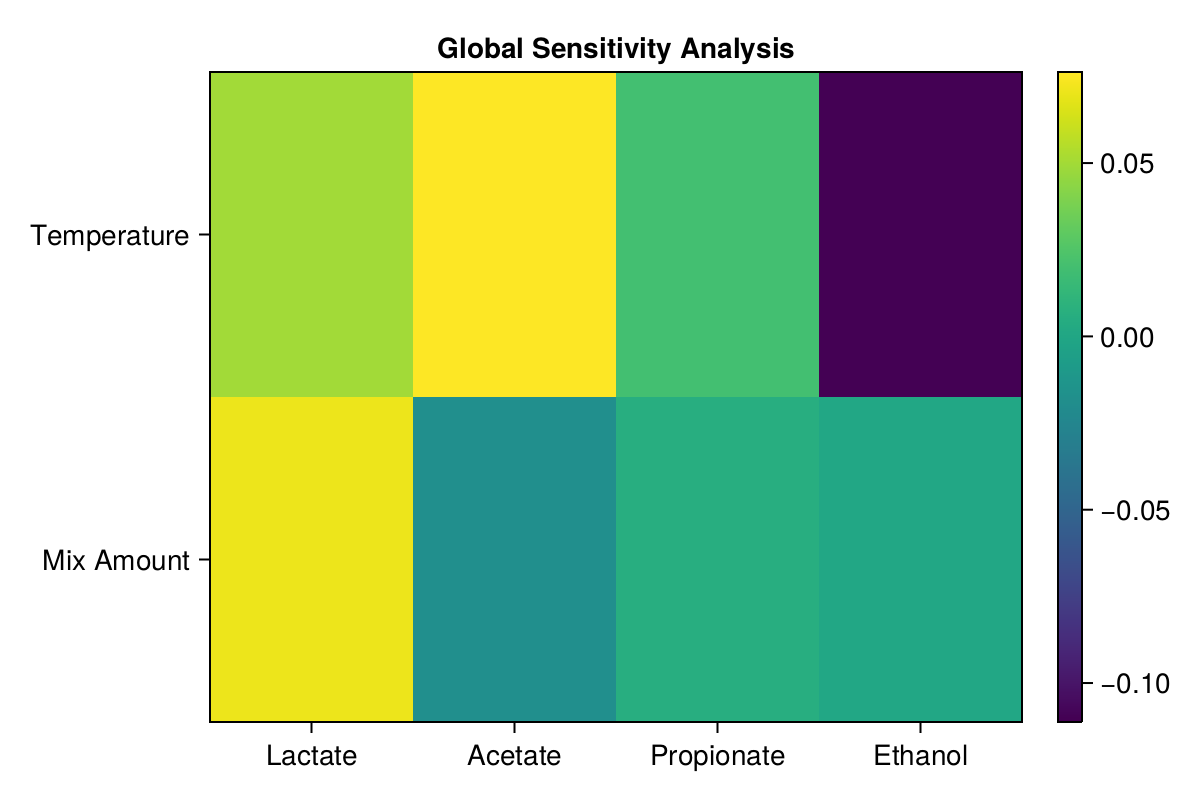
\includegraphics[width=.9\linewidth]{../plots/sensitivity/global_morris.png}
\end{center}

\begin{center}
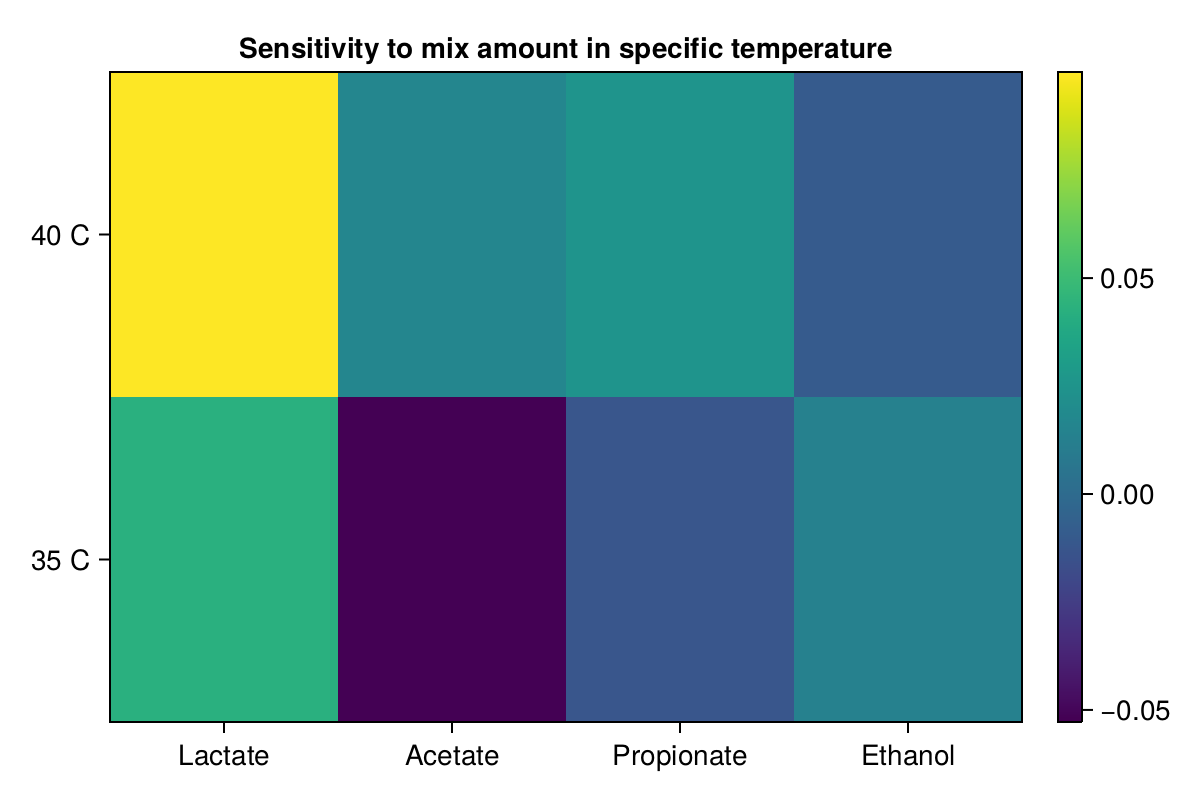
\includegraphics[width=.9\linewidth]{../plots/sensitivity/temp_morris.png}
\end{center}

\begin{center}
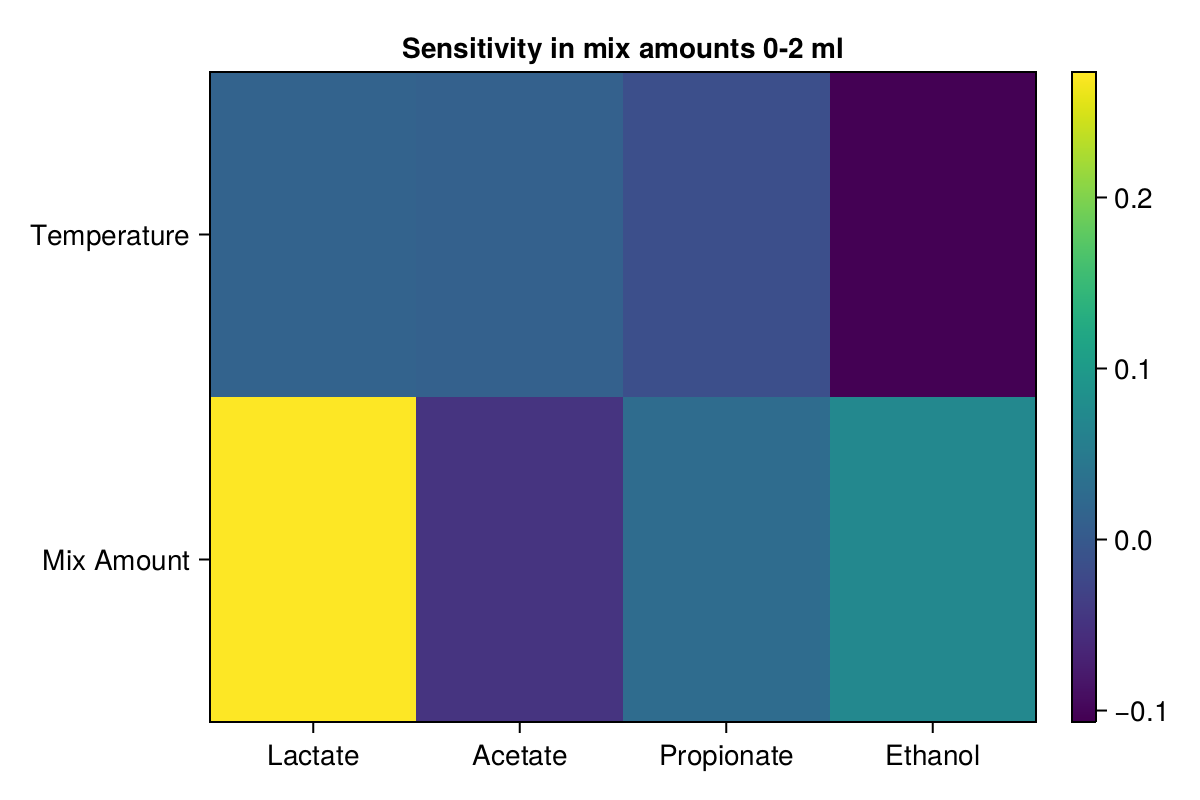
\includegraphics[width=.9\linewidth]{../plots/sensitivity/morris_low.png}
\end{center}

\begin{center}
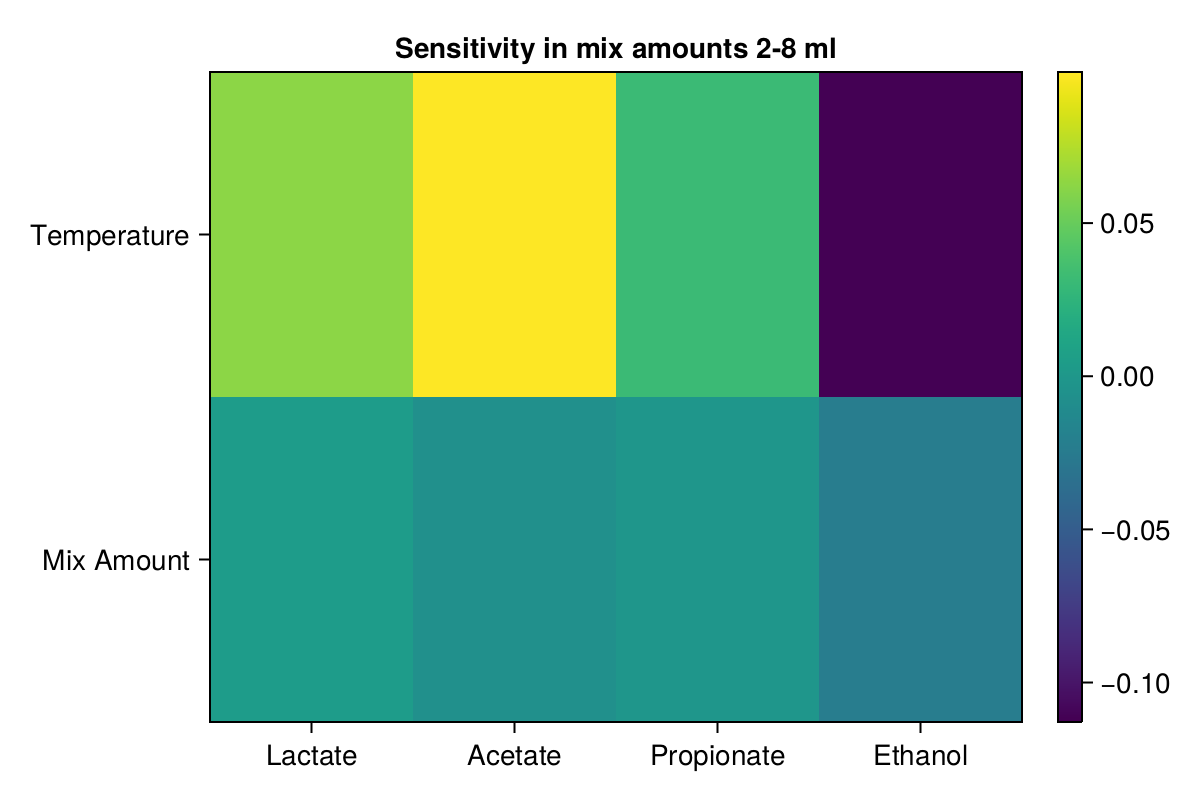
\includegraphics[width=.9\linewidth]{../plots/sensitivity/morris_high.png}
\end{center}

\subsubsection{Sobol}
\label{sec:org0bdb499}
\begin{center}
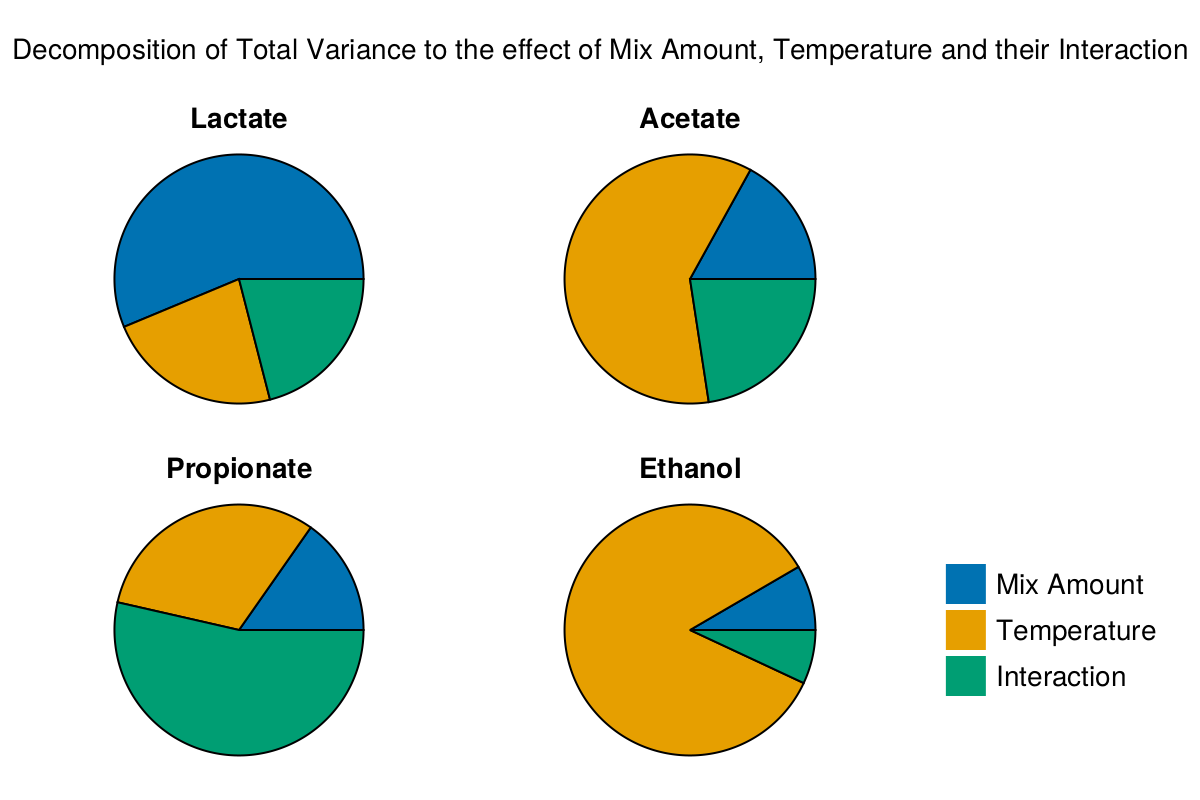
\includegraphics[width=.9\linewidth]{../plots/sensitivity/global_sobol.png}
\end{center}

\begin{center}
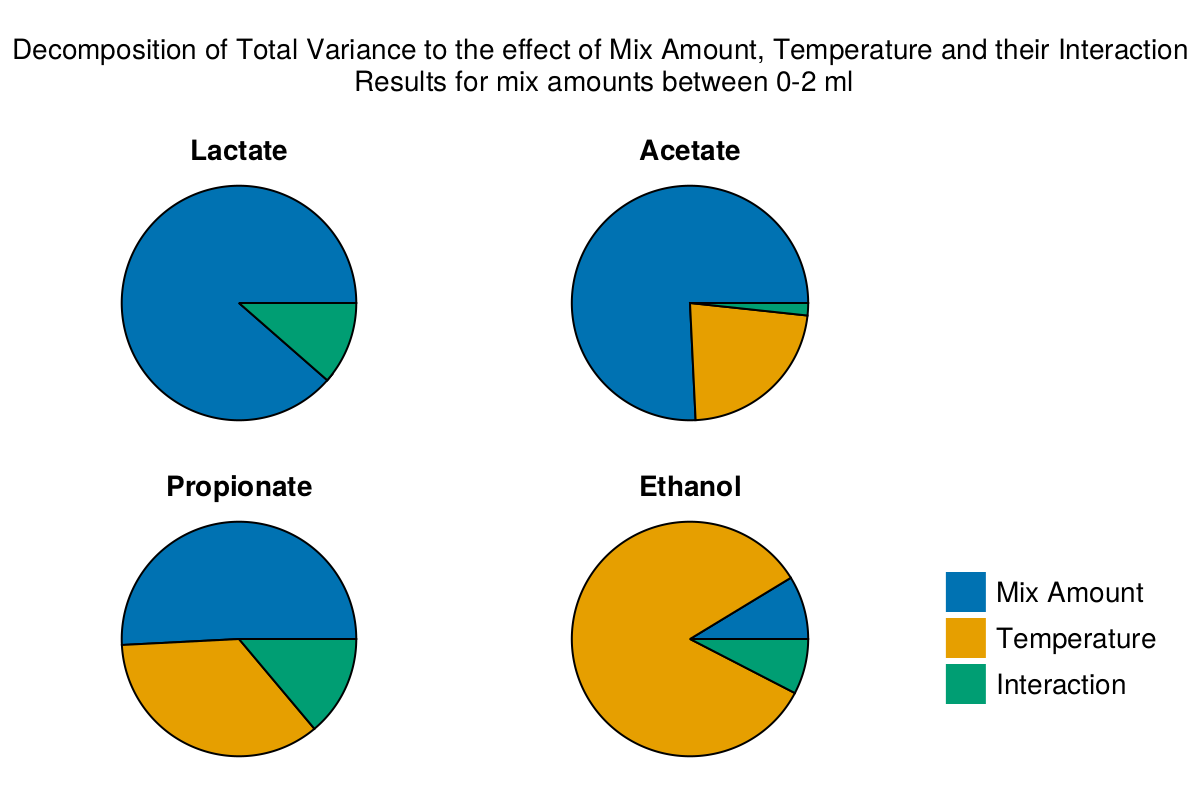
\includegraphics[width=.9\linewidth]{../plots/sensitivity/low_sobol.png}
\end{center}

\begin{center}
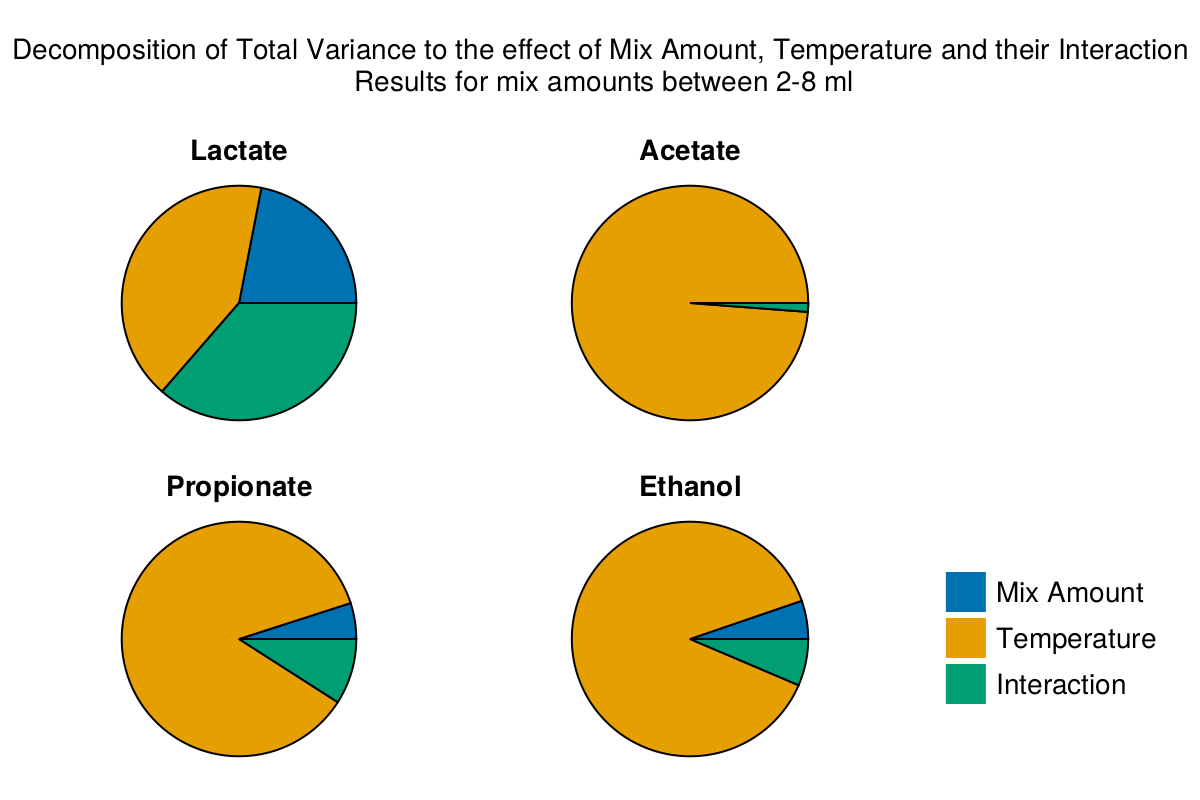
\includegraphics[width=.9\linewidth]{../plots/sensitivity/high_sobol.png}
\end{center}

\subsection{Plotting σε tornado diagrams}
\label{sec:org31f7a57}
Τα tornado diagrams είναι χρήσιμα διαγράμματα στην ανάλυση ευαισθησίας καθώς δίνουν ένα πιο εύκολο στην κατανόηση look στην ευαισθησία. Το παρακάτω code block κάνει plot τα αντίστοιχα αποτελέσματα σε ένα tornado plot. Για να γίνει αυτό, κάνουμε sort τα αποτελέσματα της ευαισθησίας μαζί με τα labels τους κατ'απόλυτη τιμή αλλά δεν κάνουμε plot την απόλυτη τιμή επειδή θέλουμε να φαίνεται πότε μία επίδραση είναι αρνητική. Έπειτα, ορίζουμε δύο χρώματα (ένα για τις θετικές και ένα για τις αρνητικές επιδράσεις) και κάνουμε plot το tornado diagram με αυτά τα στοιχεία. Αυτό επαναλαμβάνεται για όλες τις αναλύσεις που κάναμε.

\begin{minted}[breaklines=true,breakanywhere=true]{julia}

# Define the labels
name_matrix = ["Lactate - Mix Amount", "Acetate - Mix Amount", "Propionate - Mix Amount", "Ethanol - Mix Amount", "Lactate - Temperature", "Acetate - Temperature", "Propionate - Temperature", "Ethanol - Temperature"]

# Sort the data and their labels
reshaped_sens_total = reshape(total_sens2, 1:8)
sorted_indices_total = sortperm(abs.(reshaped_sens_total))

sorted_sens_total = reshaped_sens_total[sorted_indices_total]
sorted_names_total = name_matrix[sorted_indices_total]

# Define an x-range
xrange_total = LinRange(minimum(sorted_sens_total), maximum(sorted_sens_total), 8)

# Define colors based on the sign of sensitivity values
colors_total = ifelse.(sorted_sens_total .< 0, "#440154", "#DCE319")

# Create the tornado plot
global_tornado = bar(xrange_total, sorted_sens_total, color = colors_total,
                     xlabel = "Sensitivity", yticks = (xrange_total, sorted_names_total),
                     orientation = :h, legend = false,
                     title = "Tornado Diagram for Global Sensitivity Analysis",
                     size = (900, 600), tickfontsize = 12, guidefontsize = 14)
savefig(global_tornado, plotsdir("sensitivity", "global_tornado.png"))

# Do this for the low mix amount domain
reshaped_sens_low = reshape(sens_low2, 1:8)
sorted_indices_low = sortperm(abs.(reshaped_sens_low))

sorted_sens_low = reshaped_sens_low[sorted_indices_low]
sorted_names_low = name_matrix[sorted_indices_low]

# Define an x-range
xrange_low = LinRange(minimum(sorted_sens_low), maximum(sorted_sens_low), 8)

# Define colors based on the sign of sensitivity values
colors_low = ifelse.(sorted_sens_low .< 0, "#440154", "#DCE319")

# Create the tornado plot
low_tornado = bar(xrange_low, sorted_sens_low, color = colors_low,
                  xlabel = "Sensitivity", yticks = (xrange_low, sorted_names_low),
                  orientation = :h, legend = false,
                  title = "Tornado Diagram for Mix Amounts 0-2 ml",
                  size = (900, 600), tickfontsize = 12, guidefontsize = 14)
savefig(low_tornado, plotsdir("sensitivity", "tornado_low.png"))

# And the high mix amount domain
reshaped_sens_high = reshape(sens_high2, 1:8)
sorted_indices_high = sortperm(abs.(reshaped_sens_high))

sorted_sens_high = reshaped_sens_high[sorted_indices_high]
sorted_names_high = name_matrix[sorted_indices_high]

# Define an x-range
xrange_high = LinRange(minimum(sorted_sens_high), maximum(sorted_sens_high), 8)

# Define colors based on the sign of sensitivity values
colors_high = ifelse.(sorted_sens_high .< 0, "#440154", "#DCE319")

# Create the tornado plot
high_tornado = bar(xrange_high, sorted_sens_high, color = colors_high,
                     xlabel = "Sensitivity", yticks = (xrange_high, sorted_names_high),
                     orientation = :h, legend = false,
                     title = "Tornado Diagram for Mix Amounts 2-8 ml",
                     size = (900, 600), tickfontsize = 12, guidefontsize = 14)
savefig(high_tornado, plotsdir("sensitivity", "tornado_high.png"))

# We also want to do a tornado plot of the sensitivity analysis
# performed for each temperature. Theoretically, the sensitivity we
# have is how each parameter affects the system on its own, but making
# the domain smaller (studying each temperature separately) also gave
# interesting results.

name_matrix2 = ["Lactate - 35 C", "Acetate - 35 C", "Propionate - 35 C", "Ethanol - 35 C", "Lactate - 40 C", "Acetate - 40 C", "Propionate - 40 C", "Ethanol - 40 C"]

# Sort the data and their labels
reshaped_sens_temp = reshape(sens_temp, 1:8)
sorted_indices_temp = sortperm(abs.(reshaped_sens_temp))

sorted_sens_temp = reshaped_sens_temp[sorted_indices_temp]
sorted_names_temp = name_matrix2[sorted_indices_temp]

# Define an x-range
xrange_temp = LinRange(minimum(sorted_sens_temp), maximum(sorted_sens_temp), 8)

# Define colors based on the sign of sensitivity values
colors_temp = ifelse.(sorted_sens_temp .< 0, "#440154", "#DCE319")

# Create the tornado plot
temp_tornado = bar(xrange_temp, sorted_sens_temp, color = colors_temp,
                     xlabel = "Sensitivity to Mix Amount",
                     yticks = (xrange_temp, sorted_names_temp),
                     orientation = :h, legend = false,
                     title = "Tornado Diagram for Discrete Temperature Ranges",
                     size = (900, 600), tickfontsize = 12, guidefontsize = 14)
savefig(temp_tornado, plotsdir("sensitivity", "temperature_tornado.png"))
\end{minted}

Παρακάτω φαίνονται και τα αντίστοιχα plots

\begin{center}
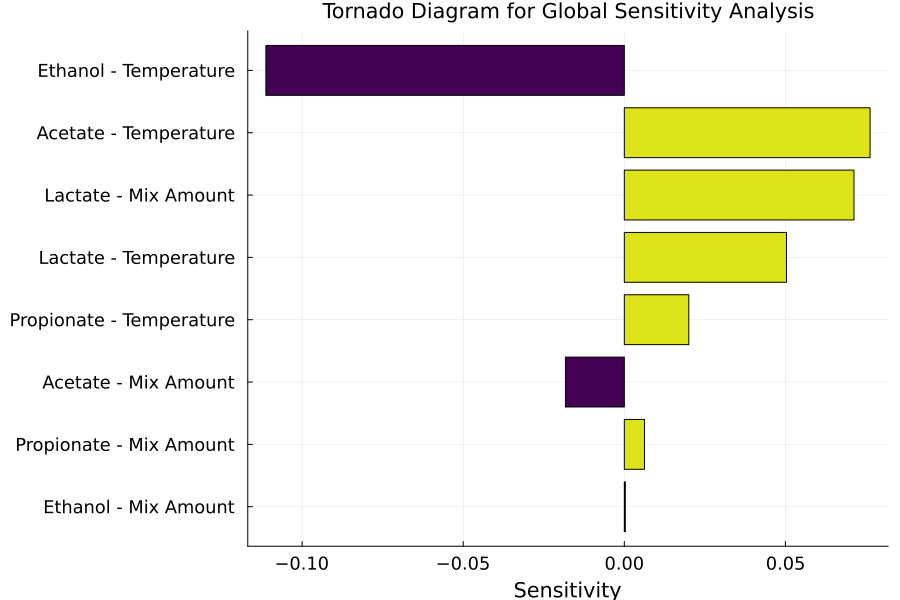
\includegraphics[width=.9\linewidth]{../plots/sensitivity/global_tornado.png}
\end{center}

\begin{center}
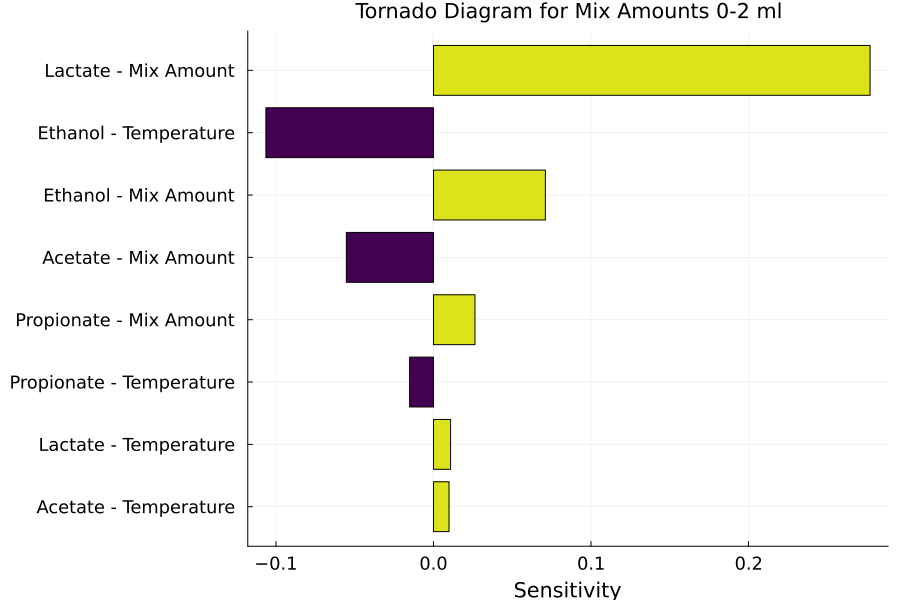
\includegraphics[width=.9\linewidth]{../plots/sensitivity/tornado_low.png}
\end{center}

\begin{center}
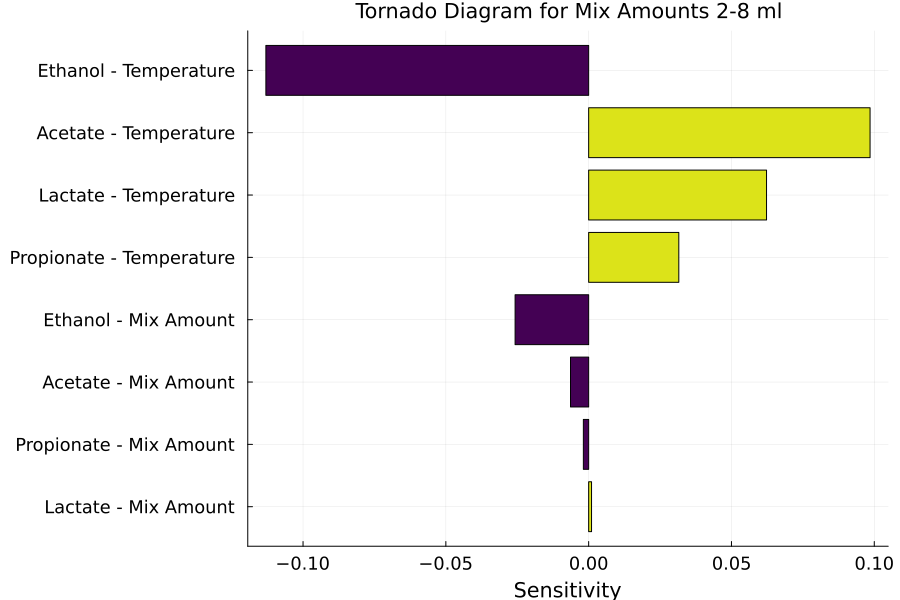
\includegraphics[width=.9\linewidth]{../plots/sensitivity/tornado_high.png}
\end{center}

\begin{center}
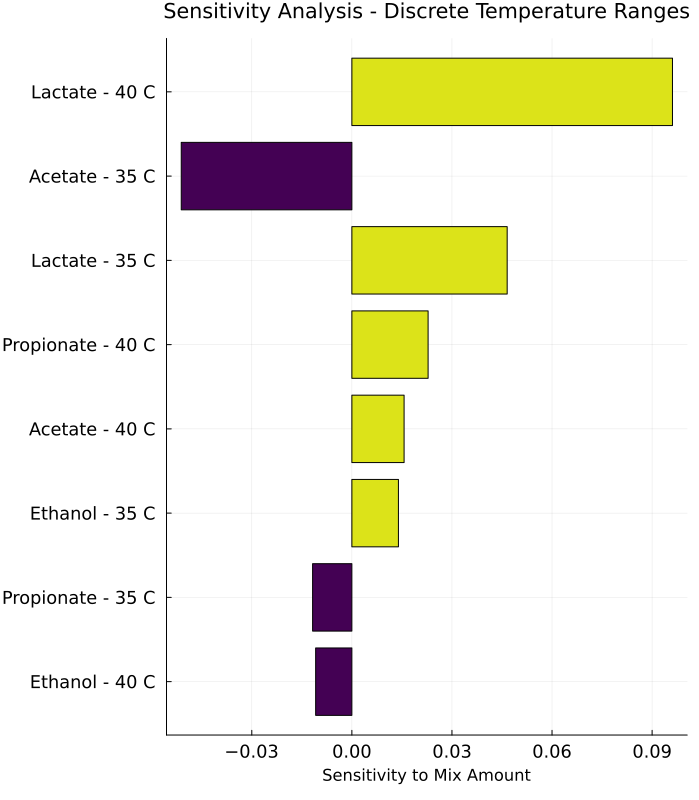
\includegraphics[width=.9\linewidth]{../plots/sensitivity/temperature_tornado.png}
\end{center}

\section{Συμπεράσματα}
\label{sec:orgd4a20bc}
Έχοντας δει πως οι μεταβολές είναι στατιστικά σημαντικές από την ANOVA, η ανάλυση ευαισθησίας αυτή μας έδωσε και κάποια ποσοτικά αποτελέσματα τα οποία μας είναι χρήσιμα.

Από την συνολική ανάλυση ευαισθησίας βλέπουμε πως το γαλακτικό οξύ έχει σχετικά μεγάλη εξάρτηση και από τις δύο παραμέτρους, αλλά επηρεάζεται περισσότερο από το mix amount. Το οξικό οξύ επηρεάζεται γενικά αρνητικά από το mix amount και θετικά από την θερμοκρασία, με την θερμοκρασία να είανι πολύ πιο καθοριστική στη μεταβλητότητα. Το προπιονικό φαίνεται να έχει ασθενή επίδραση και με τους δύο παράγοντες, όμως τα αποτελέσματα του είναι αρκετά διαφορετικά για τα δύο πειράματα, το οποίο μας οδηγεί στην σκέψη ότι η σημαντικότερη επίδραση είναι λόγω κάποιας αλληλεπίδρασης και δεν μπορεί να δωθεί στον έναν ή τον άλλο παράγοντα. Τέλος, η αιθανόλη έχει μία ισχυρή αρνητική επίδραση από την θερμοκρασία η οποία αποτελεί περίπου το 85\% της μεταβλητότητας της και στην συνολική ανάλυση φαίνεται να έχει αμελητέα επίδραση από την ποσότητα του mix.

Εξετάζοντας την περιοχή των μικρών ποσοτήτων του mix, βλέπουμε πολύ θετικότερες επιδράσεις στην αιθανόλη και το γαλακτικό. Το γαλακτικό έχει πλέον μία εξάρτηση κατά 90\% περίπου από το mix amount δείχνοντας ότι σε αυτές τις ποσότητες, και στις δύο θερμοκρασίες κάνει perform παρόμοια. Η αιθανόλη παραμένει ισχυρά αρνητικά εξαρτούμενη από την θερμοκρασία αλλά φαίνεται περισσότερο η επίδραση του mix. Το προπιονικό αποκτά και αυτό μία σημαντικότερη εξάρτηση από το mix amount, παρόλο που ακόμη δεν είναι πολύ υψηλή (50\% της συνολικής). Τέλος, το οξικό, σε αυτή την περιοχή εξαρτάται και αυτό ισχυρά από το mix amount αλλά με αρνητικό τρόπο (το οποίο στηρίζεται στην παρατήρηση ότι ιδιαίτερα στους 35, όταν βάζουμε το mix σταματάει η οξικογένεση) ενώ η επίδραση της θερμοκρασίας σε αυτό φαίνεται λιγότερο καθώς δείξαμε ότι η επίδραση της θερμοκρασίας στα 0 και 1 ml είναι οριακά σημαντική.

Στην περιοχή των μεγάλων ποσοτήτων του mix, τα αποτελέσματα συνάδουν με όσα έχουμε δείξει παραπάνω. Το οξικό, το προπιονικό και η αιθανόλη έχουν πολύ μικρή εξάρτηση από την ποσότητα του mix (μάλιστα το οξικό δείχνει να μην έχει πρακτικά καμία σε σχέση με την θερμοκρασία) και αυτή η εξάρτηση είναι και αρνητική με βάση το Morris analysis. Η εξάρτηση τους από την θερμοκρασία φαίνεται θετική για το οξικό και το προπιονικό (ειδικά του οξικού) ενώ η αιθανόλη παραμένει να έχει ισχυρή αρνητική εξάρτηση. Το γαλακτικό έχει μία θετική επίδραση από το mix amount, αλλά και αυτή δεν είναι παραπάνω από το 22\% της συνολικής του μεταβλητότητας στην περιοχή αυτή και η εξάρτηση από την θερμοκρασία είναι πιο σημαντική στην περιοχή αυτή. Οπότε, γνωρίζοντας κιόλας ότι η αύξηση της ποσότητας οδηγεί σε αύξηση του κόστους, σίγουρα δεν θα αξίζει η προσθήκη μεγαλύτερης ποσότητας από 2 ml.

Τέλος, από την ανάλυση που έγινε σε συγκεκριμένη θερμοκρασία, μπορούμε να δούμε πιο συγκεκριμένα που επηρεάζει θετικά και που αρνητικά το mix. Το γαλακτικό έχει θετική εξάρτηση και στις δύο θερμοκρασίες με αυτήν στους 40 να είναι πιο ισχυρή. Το οξικό έχει μία σχετικά μεγάλη θετική εξάρτηση στους 40 και μία σχετικά μεγάλη αρνητική στους 35. Το προπιονικό δείχνει να μην έχει πολύ μεγάλες εξαρτήσεις από το mix amount σε αυτά τα subdomains, αλλά στους 40 είναι λίγο θετική και στους 35 λίγο αρνητική ενώ το ακριβώς αντίθετο δείχνει να συμβαίνει στην αιθανόλη.

Οπότε, τα γενικά συμπεράσματα της μελέτης σχετικά με τα προιόντα μπορούν να γραφθούν συνοπτικά ως εξής:
\begin{itemize}
\item Το γαλακτικό οξύ αυξάνεται αρκετά με την αύξηση και των δύο παραμέτρων.
\item Η προσθήκη του mix στους 35 C παρεμποδίζει ισχυρά την παραγωγή οξικού οξέος, η οποία μπορεί να γίνει χωρίς το mix. Στους 40 αυτό το φαινόμενο δεν παρατηρείται, αλλά η προσθήκη του μιξ εώς 2 ml δεν προκαλεί στατιστικά σημαντική αύξηση. Για να παραχθεί αυξημένο οξικό, θέλουμε ποσότητα 4 ml και πάνω, όπου και μέχρι 8 ml, δεν υπάρχει βελτίωση σε σχέση με τα 4 ml. Και ακόμη και εκεί, η αύξηση δεν είναι τεράστια (0.1 g/l).
\item Το προπιονικό οξύ εξαρτάται μεν και από τις δύο παραμέτρους, αλλά δεν δείχνει να έχει τόσο μεγάλη αλλαγή λόγω αυτών συγκριτικά με τα άλλα προιόντα, συμπεραίνοντας ότι η συσχέτιση είναι μάλλον ασθενέστερη.
\item Η αύξηση της θερμοκρασίας στους 40 C μειώνει σημαντικά την παραγωγή αιθανόλης. Η παραγωγικότητα εξαρτάται και από την ποσότητα του μιξ που προστίθεται, αλλά αυτή η συσχέτιση είναι πολύ ασθενέστερη σε σχέση με την θερμοκρασιακή.
\end{itemize}

Στους 35 C, η βέλτιστη ποσότητα είναι τα 2 ml, τα οποία οδηγούν σε μεγάλη παραγωγικότητα γαλακτικού οξέος και αιθανόλης, καλή παραγωγή προπιονικού και μειωμένο οξικό. Λιγότερη αλλά και περισσότερη ποσότητα του μιξ μειώνει την παραγωγικότητα.

Στους 40 C, τα σημαντικά προιόντα είναι το γαλακτικό και το οξικό, καθώς η αιθανόλη είναι πολύ μειώμενη. Το γαλακτικό είναι σημαντικά περισσότερο από ότι στους 35 C. Το προπιονικό παράγεται σε παρόμοιο ρυθμό, αλλά δείχνει να έχει μία μικρή θετική εξάρτηση από την αύξηση της θερμοκρασίας. Τα 2 ml ευνοούν την παραγωγή γαλακτικού και προπιονικού σε σχέση με το να μην προστεθεί το μιξ, ενώ το οξικό δεν έχει σημαντική διαφορά. Τα 4 ml ευνοούν περαιτέρω την παραγωγή γαλακτικού και οξικού και με 95\% βεβαιότητα και του προπιονικού ενώ τα 8 ml αυξάνουν μόνο την παραγωγή γαλακτικού. Βέβαια, αξίζει να σημειωθεί πως παρότι η επίδραση αυτή είναι θετική, η ανάλυση ευαισθησίας έδειξε ότι ένα πολύ μικρό κομμάτι της πιθανής μεταβλητότητας αφορά την ποσότητα του μιξ όταν αυτά είναι από 2 ml και πάνω, οπότε συγκρίνοντας το με το κόστος, πιθανόν να μην αξίζει.

Οπότε, σε κάθε περίπτωση, εκτός αν μας ενδιαφέρει η αυξημένη συγκέντρωση αιθανόλης, η λειτουργία στους 40 C είναι καλύτερη και η ποσότητα που προτιμάται είναι τα 4 ml αν πάμε καθαρά για τα μέγιστα προιόντα, αλλά λόγω του οικονομικού tradeoff, είναι πιθανό να αξίζει περισσότερο και τα 2 ml.

Αξίζει επίσης να σημειωθεί ότι από το ένα προπαρασκευαστικό πείραμα που έγινε στους 45 C, ξέρουμε πως σε εκείνη την θερμοκρασία, η αιθανόλη παραμένει χαμηλή αλλά τώρα και το γαλακτικό καταναλώνεται εις βάρος του οξικού και του προπιονικού. Λόγω του διαφορετικού τρόπου διεξαγωγής του πειράματος αυτού, δεν θεωρείται έγκυρο να συγκριθεί με το πείραμα στους 40 ποσοτικά, αλλά αυτό μας δίνει μία ένδειξη πως κάποια θερμόφιλη ομάδα μικροοργανισμών μπορεί να διασπάσει το γαλακτικό οξύ. Γνωρίζουμε από την βιβλιογραφία ότι στο μονοπάτι παραγωγής του προπιονικού οξέος, το πυροσταφυλικό γίνεται γαλακτικό και μετά προπιονικό και παρόλα αυτά, μόνο στους 45 έχουμε παρατηρήσει την μείωση του γαλακτικού, οπότε αυτή η θερμόφιλη αντίδραση που γίνεται στους 45 και πάνω είναι μάλλον αντίδραση οξικογένεσης. Πιθανόν κάποιο μέρος να πηγαίνει και σε προπιονικό, αλλά με βάση τα άλλα πειράματα, το σημαντικό ποσοστό πηγαίνει στην οξικογένεση.
\end{document}